%% Template for EU report, using the report.sty style file

\documentclass[12pt,a4paper,twoside]{article}
%% common package
\usepackage[headers]{report}
\usepackage{xspace}
\usepackage{verbatim}
\usepackage[usenames]{color}
\usepackage[usenames,dvipsnames,table]{xcolor}
\usepackage[pdftex,dvips]{graphicx}
\usepackage{url}
\usepackage{array}
\usepackage{color}
\usepackage{longtable}
\usepackage{amsmath}
\usepackage{bm}
\usepackage[T1]{fontenc}
\usepackage{lmodern}
\usepackage{textcomp}

\renewcommand{\labelenumii}{\theenumii}
\renewcommand{\theenumii}{\theenumi.\arabic{enumii}.}

%%

%%insert here other packages needed by sections

%%

%%%%%%%%%%%%%%%%%%%%%%%%%%%%%%%%%%%%%%%%%%%%%%%%%%%%%%%%%%%%%%%%%%%%%%%%%%%%%%
%%% Titlepage
%%%%%%%%%%%%%%%%%%%%%%%%%%%%%%%%%%%%%%%%%%%%%%%%%%%%%%%%%%%%%%%%%%%%%%%%%%%%%%

% declaration of variables used in style
\reportDocnumber{Final report}
\reportTitle{Final project objectives report}

\reportAuthor{CoDyCo Consortium}
\reportResponsiblePartner{IIT}
\reportAffiliation{% Insert here authors affiliations
 IIT, TUD, UPMC, UB, JSI.
}

\reportReviewer{}
\reportCoordinator{Francesco Nori}
\reportActivityNumber{1} %% n=1,..,10
\reportActivity{RTD}
\reportDoctype{Periodic report} %% or Prototype
\reportClassification{Public} % or Consortium
\reportDistribution{Consortium} %
\reportStatus{Draft} % Draft or Final
\reportDeliveryDate{28/04/2017}
\reportVersion{1.0}
\reportDate{Apr.~28, 2017}
\reportYear{2017}
\reportPages{\pageref{LastPage}}
\reportChangelog{v.1.0 & Feb 13, 2017 & First draft %%\\\hline
%%              v.2.0 & Feb 20, 2007 & Final version
}
\reportProjectStartingDate{1st March 2017}
\reportProjectEndDate{28th March 2017}
\reportProjectAcronym{CoDyCo}
\reportProjectTitle{Whole-Body Compliant Dynamical Contacts in Cognitive Humanoids}
 \reportContractNumber{600716}
 \reportProjectCoordinator{Istituto Italiano di Tecnologia}
 \reportProjectUrl{www.codyco.eu}
 \reportFrameworkProgramme{FP7}
 
 \reportWorkpackage{All work packages}
 \reportEditors{Francesco Nori, Vincent Padois, Jan Peters, Jan Babic, Michael Mistry, Serena Ivaldi, Elmar Rueckert}
 \reportContributors{Entire CoDyCo consortium}
 \reportReviewers{-}
\reportAbstract{The scope of the current report is to present the results ...}
\reportReviewers{reviewers}
\reportKeywordList{kw, list, etc, }

%%%%%%%%%%%%%%%%%%%%%%%%%%%%%%%%%%%%%%%%%%%%%%%%%%%%%%%%%%%%%%%%%%%%%%%%%%%%%%
%%% Sections
%%%%%%%%%%%%%%%%%%%%%%%%%%%%%%%%%%%%%%%%%%%%%%%%%%%%%%%%%%%%%%%%%%%%%%%%%%%%%%

%% constants{}

%%%%%%%%%%%%%%%%%%%%%%%%%%%%%%%%%%%%%%%%%%%%%%%%%%%%%%%%%%%%%%%%%%%%%%%%%%%%%%
%%% Misc. by Vincent
%%%%%%%%%%%%%%%%%%%%%%%%%%%%%%%%%%%%%%%%%%%%%%%%%%%%%%%%%%%%%%%%%%%%%%%%%%%%%%
\usepackage{titlesec}
\newcommand{\sectionbreak}{}
\graphicspath{{./images/}}
\usepackage{pdfpages}
\usepackage{caption}
\usepackage{subcaption}
\usepackage{multirow}
\usepackage{appendix}
\usepackage{hyperref}
\hypersetup{
    bookmarks=true,         % show bookmarks bar?
    unicode=false,          % non-Latin characters in Acrobat’s bookmarks
    pdftoolbar=true,        % show Acrobat’s toolbar?
    pdfmenubar=true,        % show Acrobat’s menu?
    pdffitwindow=false,     % window fit to page when opened
    pdfstartview={FitH},    % fits the width of the page to the window
    pdftitle={yearReport.pdf},    % title
    pdfauthor={Francesco Nori},     % author
    pdfsubject={Year 4 report for the CODYCO project},   % subject of the document
    pdfcreator={Francesco Nori},   % creator of the document
    pdfproducer={Francesco Nori}, % producer of the document
    pdfkeywords= {}, % list of keywords
    pdfnewwindow=true,      % links in new window
    colorlinks=true,       % false: boxed links; true: colored links
    linkcolor=black,          % color of internal links (change box color with linkbordercolor)
    citecolor=black,        % color of links to bibliography
    filecolor=black,      % color of file links
    urlcolor=black           % color of external links
}

%%

%% Morteza's math
\newcommand{\Bc}{\mathbf{c}}
\newcommand{\BJ}{\mathbf{J}}
\newcommand{\BW}{\mathbf{W}}
\newcommand{\Bq}{\mathbf{q}}
\newcommand{\R}{\mathcal{R}}
\newcommand{\Btau}{\boldsymbol{\tau}}


%%%%%%%%%%%%%%%%%%%%%%%%%%%%%% BEGIN DOCUMENT
\begin{document}

\reportMaketitle


%%TODO move to style
\newcolumntype{L}[1]{>{\raggedright\let\newline\\\arraybackslash\hspace{0pt}}m{#1}}
\newcolumntype{C}[1]{>{\centering\let\newline\\\arraybackslash\hspace{0pt}}m{#1}}
\newcolumntype{R}[1]{>{\raggedleft\let\newline\\\arraybackslash\hspace{0pt}}m{#1}}

\clearpage

\setcounter{tocdepth}{5}

\tableofcontents

%%%%%%%%%%%%%%%%%%%%%%%% Start report content here.

\section{Project objectives}

\subsection{Overview}

The specificity of CoDyCo relies on the fact that the progress beyond the state of the art is guided by the yearly implementation on the iCub humanoid. Within this context, iCub is a peculiar platform being the only humanoid integrating whole-body distributed force and tactile sensors. In this sense CoDyCo specific objectives were to design and implement the control of whole-body posture during physical human robot interaction. Other long term objectives involve setting up the necessary infrastructure (human experimental protocols, software infrastructure, learning and control specifications) for leveraging the activities in previous years. 

The aim of CoDyCo was to advance the control and cognitive understanding about robust, goal- directed whole-body motion interaction with multiple contacts. When the CoDyCo consortium wrote the project milestones, our goal was to go beyond traditional approaches. First, we wanted to propose methodologies for performing coordinated interaction tasks with complex systems. Second, to combine planning and compliance to deal with predictable and unpredictable events and contacts. Finally, we wanted to do something to validate theoretical advances in real-world interaction scenarios.

\subsection{Overview WP2: what we learn from humans }

To guide robotic developments within Codyco, we performed a series of human behavioural experiments. We recorded human subjects undergoing a set of whole body motions involving contacts with different types of environment. The set included balancing with multiple rigid contacts, goal directed actions involving supportive hand contacts while balancing on surfaces of different stability, learning to use non-rigid contacts and human assistive contact. These experiments, and the resulting data were essential for the robotic developments and provided the consortium with the guiding principles for designing robot control policies and principles for physical interaction between the robots, humans, and the environment.

To guide robotic developments within Codyco, we performed a series of human behavioural experiments. 
We recorded human subjects undergoing a set of whole body motions involving contacts with different types of environment. The set included balancing with multiple rigid contacts, 
goal directed actions involving supportive hand contacts while balancing on surfaces of different stability, learning to use non-rigid contacts and human assistive contact. These experiments, and the resulting data were essential for the robotic developments 
and provided the consortium with the guiding principles for designing robot control policies 
and principles for physical interaction between the robots, humans, and the environment. 


\subsection{Overview WP1: tools for describing the motion}
To facilitate collaboration between CoDyCo partners, we set out from the very beginning of the project, to develop a common set of software tools shared amongst all members.  The tools we developed include methods for modelling, simulating and calibrating whole body robot behaviours with contact interactions, but importantly also for modeling human motion with contact interaction. We believe that there are underlying principles that may be applied to understanding both human and robot motion, and having a common set of tools to work with helps us draw those connections.   

\subsection{Overview WP5: porting the results on the iCub}

The project achievements were validated on the iCub. iCub is a humanoid robot with the size of a 4 years old child. The robot is equipped with numerous sensors that makes it unique: it has inertial sensing in the head, which acts like our vestibular system; then force/torque sensing in the arms, legs and feet, and an artificial skin consisting of distributed tactile sensors. Thanks to all these sensors, we can compute in real-time the forces that the robot exchange with the human or the environment when there is a contact on its body.

The experimental validation of the controllers developed during the CoDyCo journey has required not only a deep understanding of the theoretical framework, but also a clear insight into the iCub software infrastructure and into the so called low-level. In fact, controllers usually provide the robot with high-level objectives such as balancing and compliance during user interaction. These high level objectives must be translated into nested, consequent objectives until the commands we send to the robot motors. Hence, actuation modelling, tuning, efficient controller implementation, and iterative optimization of the obtained performances have been key ingredients for the success of the CoDyCo demos. More importantly, the implementation of control algorithms on the iCub platform has served as a tool for the theoretical investigations that we had to pursue. For example, after implementing state -of-the art control algorithms we observed that some of these were simply unstable. We then focused on how to modify these algorithms to obtain stability, a fundamental property for whole body controllers.

\subsection{Overview WP3: the controller that we use}

Controlling humanoids in situations where multiple contacts have to be made with the environment in order to maintain or improve balance is a complex problem. This complexity is mostly due to two factors. The first one relates to the complexity of the system and of its interaction with the environment. Indeed the problem has to be looked at from a dynamics point of view where interaction forces can be accounted for. This requires an accurate knowledge of the robot model,  the fine-tuning of low-level control loops, a correct estimation of interaction forces with the environment and more generally of the system's state as well as the capability to strictly respect constraints acting on the system while achieving several tasks at the same time. The second factor is related to the hybrid nature of humanoids. Humanoids are intrinsically underactuated systems which can compensate for underactuation through unilateral physical interactions with their environment. Unilaterality means that contacts can be made and broken. Deciding when and where to break/make contact is a complex problem as it involves a preview of the effect of this discrete decision over a time horizon. In CoDyCo we  provide robust and generic control approaches to tackle the complexity of this control problem.

\subsection{Overview WP4: why and where we use learning}

Autonomous robots that can assist humans in situations of daily life have been a long standing vision of robotics, artificial intelligence, and cognitive sciences. A first step towards this goal is to create robots that can learn tasks triggered by visual stimuli from higher level instruction. However, learning techniques have yet to live up to this promise as only few methods manage to scale to high-dimensional manipulator or humanoid robots.We investigate the key ingredients for learning motor skills in robotics including both manipulation of static and dynamic objects that are perceived using vision or tactile sensing. The resulting approach relies on a representation of motor skills by parameterized motor primitive policies acting as building blocks of movement generation, and a learned task execution module that transforms these movements into motor commands. We discuss task-appropriate learning approaches for imitation learning, model learning and reinforcement learning for robots with many degrees of freedom that perceive the manipulated objects using robot vision or tactile sensing. Empirical evaluations on our iCub  illustrate the effectiveness and applicability to learning control when making and breaking contact with the environment.

\subsection{Overview: conclusion}

After four years of intensive activities, the CoDyCo consortium achieved an outstanding number of advances in the field of controlling and cognitive understanding about robust, goal-directed whole-body motion interaction with multiple contacts. Thanks to experiments with humans coordinated by Jan Babic at JSI and modeled by Mike Mistry at UB, we were able to develop novel metrics to understand when humans proficiently exploit whole-body distributed contacts. Theoretical advances in the field of control achieved by Vincent Padois at UPMC, gave robots the ability to control their whole-body posture by means of contact force regulation. Learning strategies have been coordinated by Jan Peters at TUD and gave robots the ability to adapt their control actions on the basis of human requirements. Implementation on the iCub humanoid have validated the utility of the conducted research on real-world scenarios.

\section{Progress overview and contribution to the research field}

All the CoDyCo objectives have been attained. Here is a list of the CoDyCo achievements. 
\begin{enumerate}
 
\item First year achievements:
\begin{enumerate}
\item Design and implementation of an open-source simulator environment for the iCub and digital human whole-body motion simulation. After a consortium shared effort, it was decided to adopt Gazebo \url{http://gazebosim.org} as a basis for the simulator. Gazebo offers a structured software interface (plugins) which was used to export a YARP interface to simulated robots. The Gazebo-YARP plugin source code is available on github, at the address \url{https://github.com/robotology/gazebo_yarp_plugins}. The use of Gazebo was chosen on the basis of a public survey \url{http://arxiv.org/abs/1402.7050} and on the results of a discussion conducted in Paris during a workshop organized at ISIR.

\item Design and implementation of a whole-body software abstraction layer \url{https://github.com/robotology/codyco/tree/master/src/libraries/wholeBodyInterface} which represents the backbone of the CoDyCo software architecture, interface and module structure.

\item Design and definition of human experimental protocols and simplified models for whole-body motion with multiple contacts. After an extensive literature review (D2.1), JSI conducted preliminary studies on examining functional role of supportive hand contact while balancing.

\item Design and test of state of the art control strategies for whole-body motion with multiple contacts. Realization of a solver for the whole-body reactive control that provides an expressive and rich description of the control problem as well as an efficient way of solving it. Implementation of the results in a whole-body control validation scenario in presence of multiple contacts. 

\item Preliminary studies on learning methods suitable for tasks that involve many uncertain contacts. Design of fast regression methods that can deal with well structured input noise. Methods for learning how to combine elementary control tasks.
\end{enumerate}

\item Second year achievements: 

\begin{enumerate}

\item Design, implementation and maintenance of the whole-body control software infrastructure. The infrastructure consists of several modules which significantly improved the controller accuracy and robustness thanks to: a module for whole-body torques estimation, a module for force/torque sensors calibration, a module for whole-body dynamics identification and a module for dynamics estimation. 

\item Design of experimental protocols and data collection of experiments for studying humans in multi-contact interaction with the environment. This includes an experiment on hand-contact assisted balancing, a metric for whole-body stability characterisation, an experiment of human robot physical interaction and a study on collaborative human-robot physical interaction.

\item Design and simulation of whole-body control strategies in presence of non-rigid contacts. Experiments on postural control under multiple environmental contacts while controlling the operational space dynamics. 

\item Development of a theoretical framework for representing movement primitives within probabilistic contexts. Design of a model-free probabilistic representation for simultaneous representation of kinematic and force trajectories. Preliminary studies on the problem of learning strategies to adapt temporal activation of low-level primitives and to deal with interferences in combining multiple whole-body tasks. 

\item Implementation of the second year validation scenario consisting in whole-body motion control subject to postural, contact and goal-directed (Cartesian) constraints.

\end{enumerate}

\item Third year achievements:

\begin{enumerate}

\item Release of an open-source software for contact compliance estimation.

\item Release of an open-source software for floating-base estimation.

\item Models of human interaction with compliant contacts.

\item Definition and solution of the theoretical framework for balancing on compliant contacts.

\item Learning models of simultaneous use of elementary tasks and co-articulation of multiple tasks.

\item Implementation of the third validation scenario: balancing on compliant or dynamical contacts.

\end{enumerate}

\item Fourth year achievements:
\begin{enumerate}
\item Real-time estimation of human and robot kinematics and dynamics during physical human-robot interaction. 

\item Experiments of human whole-body dynamics during goal-directed tasks with contacts. A memory task and an inhibitory Stroop task were performed to explore cognitive control over balance in novel challenging conditions.

\item Control algorithm based on incremental task compatibility optimization to allow incremental adaptation of operational tasks during whole-body control. 

\item Probabilistic movement representation of skills to learn task prioritization from human demonstrations. 
\end{enumerate}
\end{enumerate}

\section{Management}

The CoDyCo project was managed successfully. Management activities included three amendments, smoothly organized by the consortium and the project officer. Specifically, an amendment was necessary to include INRIA among the partners. Finances were smoothly organized with no significant modifications with respect to the original plan. Several scientific publications have been achieved within the project. Dissemination events included summer schools, TV shows participations and invited talks at scientific events.

\subsection{WP1 effort summary}
Planned. the use of resources within WP1 was in accordance to the plans. 

\begin{center}
  \begin{tabular}{|C{1.5cm}|C{1.5cm}|C{1.5cm}|C{2cm}|C{2cm}|C{2cm}|C{2cm}|}
    \hline \footnotesize \textbf{WP1 person months}& \footnotesize
    \textbf{IIT}&\footnotesize \textbf{TUD}&\footnotesize \textbf{UPMC}&
    \footnotesize \textbf{UB} &\footnotesize \textbf{JSI} & \footnotesize \textbf{INRIA}\\
    \hline \footnotesize Year 1  & 8.67  & 1.00 & 3.29 & 0.51 & 2.00 & -\\
    \hline \footnotesize Year 2  & 3.00  & 3.00 & 0.47 & 2.29 & -    & - \\
    \hline \footnotesize Year 3  & -     & 1.00 & -    & 2.18 & 2.00 & 2.96 \\
    \hline \footnotesize Year 4  & -     &  1.00 &  1.44 &  2.45  &  2.00  &  2.06 \\ \hline 
    \footnotesize Total & 11.67 &  6.00 &  5.20 &  7.43 &  6.00 &  5.02    \\  \hline
    \hline \footnotesize Planned & 12.00 & 9.00 & 6.00 & 15.00 & 6.00 & 5.00 \\
    \hline
  \end{tabular}
\end{center}

\subsection{WP2 effort summary}
Planned, the use of resources within WP2 was in accordance to the plans. There was an increase in the amount of PM for JSI due to the fact that we hired PhD students instead of a more efficient post-doc.
\begin{center}
\begin{tabular}{|C{1.5cm}|C{1.5cm}|C{1.5cm}|C{2cm}|C{2cm}|C{2cm}|C{2cm}|}
\hline
\footnotesize \textbf{WP2 person months}& \footnotesize \textbf{IIT}&\footnotesize \textbf{TUD}&\footnotesize \textbf{UPMC}& \footnotesize \textbf{UB} &\footnotesize \textbf{JSI} & \footnotesize \textbf{INRIA} \\ \hline
\footnotesize Year 1  &  -     & -    & 0.28 & 2.64  & 18.80  & -     \\  \hline
\footnotesize Year 2  &  -     & 3.00 & 0.48 & 7.67  & 21.85  & -     \\  \hline
\footnotesize Year 3  &  -     & 1.00 & 1.20 & 13.88 & 21.69  & 0.52  \\  \hline
\footnotesize Year 4  &  0.00  &  3.00 &  0.75 &  25.43 &  21.62 &  1.00  \\  \hline 
\footnotesize Total & 0.00 &  7.00 &  2.71 &  49.62 &  83.96 &  1.52     \\
\hline \hline
\footnotesize Planned & -      & 4.00 & 1.00 & 45.00  & 55.00 & 1.00  \\  \hline
\end{tabular}
\end{center}

\subsection{WP3 effort summary}
\begin{center}
\begin{tabular}{|C{1.5cm}|C{1.5cm}|C{1.5cm}|C{2cm}|C{2cm}|C{2cm}|C{2cm}|}
\hline
\footnotesize \textbf{WP3 person months} & \footnotesize \textbf{IIT}&\footnotesize \textbf{TUD}&\footnotesize \textbf{UPMC}& \footnotesize \textbf{UB} &\footnotesize \textbf{JSI} &\footnotesize \textbf{INRIA} \\ \hline
\footnotesize Year 1  &  9.90 & 4.60  & 15.15 & -    & -    &  -   \\  \hline
\footnotesize Year 2  &  -    & 10.5  & 14.67 & 1.85 & 1.00 & 4.14  \\  \hline
\footnotesize Year 3  &  -    & 9.65  & 8.79  & 1.63 & 2.00 & 4.03 \\  \hline
\footnotesize Year 4  & -     &  5.60 &  8.51 &  7.15  &  1.00  &  1.98    \\    \hline
\footnotesize Planned & 9.90 &  30.35 &  47.12 &  10.63 &  4.00 &  10.15    \\
\hline \hline
\footnotesize Planned &  9.00 & 24.00 & 43.5 & 10.00 & 4.00 & 10.50 \\ \hline
\end{tabular}
\end{center}


\subsection{WP4 effort summary}
\begin{center}
\begin{tabular}{|C{1.5cm}|C{1.5cm}|C{1.5cm}|C{2cm}|C{2cm}|C{2cm}|C{2cm}|}
\hline
\footnotesize \textbf{WP4 person months}& \footnotesize \textbf{IIT}&\footnotesize \textbf{TUD}&\footnotesize \textbf{UPMC}& \footnotesize \textbf{UB} &\footnotesize \textbf{JSI} &\footnotesize \textbf{INRIA}\\ \hline
\footnotesize Year 1  &  -        & 8.00   & 2.22 & -       & -        & -     \\  \hline
\footnotesize Year 2  &  6.04  & 21.70 & 1.69 & 2.15 & 3.00   & 2.01     \\  \hline
\footnotesize Year 3  &  9.79  & 12.00 & 0.74 & 1.68 & 3.00   & 3.30 \\  \hline
\footnotesize Year 4  & 15.80 &  9.50 &  1.87 &  1.59  &  4.00  &  4.02    \\  \hline
\footnotesize Total  & 31.63 &  51.20 &  6.52 &  5.42 &  10.00 &  9.33    \\
\hline \hline
\footnotesize Planned & 30.00 & 38.00 & 9.00 & 12.00&10.00 & 9.00 \\ \hline
\end{tabular}
\end{center}

\subsection{WP5 effort summary}
\begin{center}
\begin{tabular}{|C{1.5cm}|C{1.5cm}|C{1.5cm}|C{2cm}|C{2cm}|C{2cm}|C{2cm}|}
\hline
\footnotesize \textbf{WP5 person months}& \footnotesize \textbf{IIT}&\footnotesize \textbf{TUD}&\footnotesize \textbf{UPMC}& \footnotesize \textbf{UB} &\footnotesize \textbf{JSI} & \footnotesize \textbf{INRIA} \\ \hline
\footnotesize Year 1  &  2.00  & -    & 0.31 & -    & - & -     \\  \hline
\footnotesize Year 2  &  12.00 & 0.85 & 0.05 & -    & - & -     \\  \hline
\footnotesize Year 3  &  13.06 & 2.00 & 0.14 & 1.44 & - & 0.52 \\ \hline
\footnotesize Year 4  & 16.86 &  2.00 &  1.55 &  -     &  -     &  0.99 \\   \hline
\footnotesize Total & 43.92 &  4.85 &  2.05 &  1.44 &  0.00 &  1.51    \\
\hline \hline
\footnotesize Planned &  48.00 & 5.00 & 2.50 & - & - & 1.50 \\ \hline
\end{tabular}
\end{center}

\subsection{WP6 effort summary}
Resources were used as follows.

\begin{center}
\begin{tabular}{|C{1.5cm}|C{1.5cm}|C{1.5cm}|C{2cm}|C{2cm}|C{2cm}|C{2cm}|}
\hline
\footnotesize \textbf{WP6 person months}& \footnotesize \textbf{IIT}&\footnotesize \textbf{TUD}&\footnotesize \textbf{UPMC}& \footnotesize \textbf{UB} &\footnotesize \textbf{JSI} & \footnotesize \textbf{INRIA} \\ \hline
\footnotesize Year 1 &  1.46 & - & 0.25 & - & - & -    \\  \hline
\footnotesize Year 2 &  1.50 & - & 0.31 & - & - & -     \\  \hline
\footnotesize Year 3 &  1.51 & 1.00 & 0.19 & - & 0.44 & - \\ \hline
\footnotesize Year 4  & 1.72  &  -    &  0.19 &  -     &  2.02  &  -  \\   \hline
\footnotesize Total & 6.19  &  1.00 &  0.94 &  0.00  &  2.46 &  0.00    \\
\hline \hline
\footnotesize Planned &  5.00 & 1.00 & 1.00 & 0.60 & 1.00 & - \\ \hline
\end{tabular}
\end{center}

\subsection{WP7 effort summary}
Resources were used as follows.

\begin{center}
\begin{tabular}{|C{1.5cm}|C{1.5cm}|C{1.5cm}|C{2cm}|C{2cm}|C{2cm}|C{2cm}|}
\hline
\footnotesize \textbf{WP7 person months}& \footnotesize \textbf{IIT}&\footnotesize \textbf{TUD}&\footnotesize \textbf{UPMC}& \footnotesize \textbf{UB} &\footnotesize \textbf{JSI} & \footnotesize \textbf{INRIA} \\ \hline
\footnotesize Year 1 &  1.00 & -    & 0.40 & -    & -    & - \\  \hline
\footnotesize Year 2 &  -    & -    & 0.13 & -    & -    & 0.91 \\  \hline
\footnotesize Year 3 &  1.00 & - & 0.11 & - & - & - \\ \hline
\footnotesize Year 4  & 0.50  &  1.00 &  -    &  -     &  1.00  &  1.07    \\  \hline
\footnotesize Total & 2.50 &  1.00 &  0.64 &  0.00 &  1.00 &  1.98    \\
\hline \hline
\footnotesize Planned & 3.00 & 1.00 & 1.00 & 1.00 & 1.00 & 1.00 \\ \hline
\end{tabular}
\end{center}

\section{Dissemination}

\begin{figure}
  \centering
    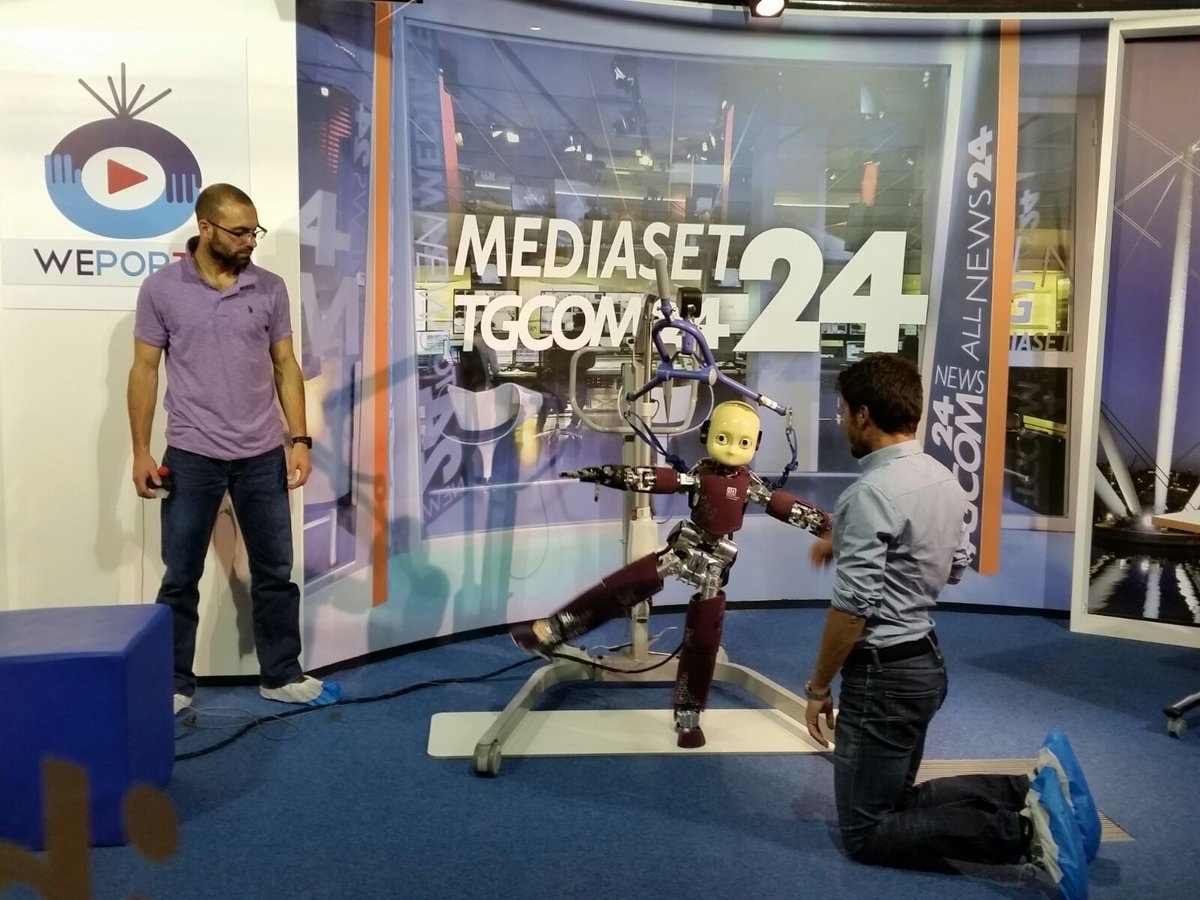
\includegraphics[height=.25\textwidth]{images/tg24}
    \hspace{1cm}
    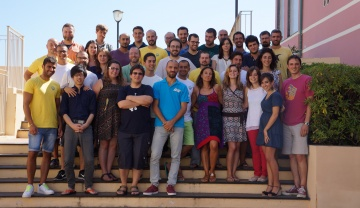
\includegraphics[height=.25\textwidth]{images/vvv}
  \caption{Dissemination of the CoDyCo project was conducted through several events. The left image refers to the
  live event on October 17th, 2016. TgCom24, live tv show on the Italian national channel. The right image refers to one of the organised summer schools (vvv14, vvv15, vvv16, vvv17). }
\end{figure}

\begin{figure}
  \centering
    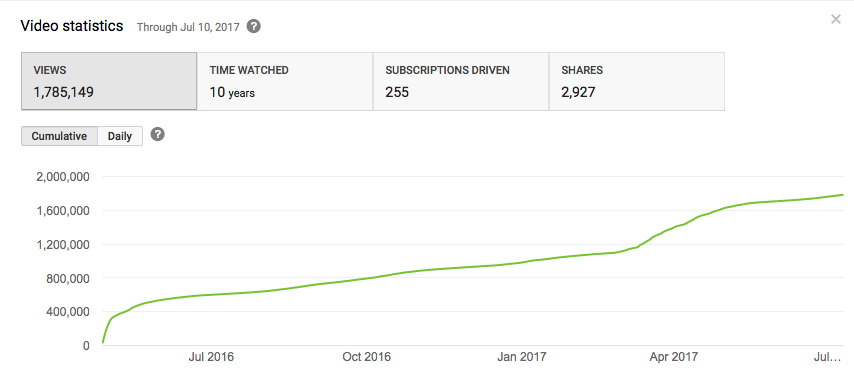
\includegraphics[height=.2\textwidth]{images/icub_igt_stats}
    \hspace{1cm}
    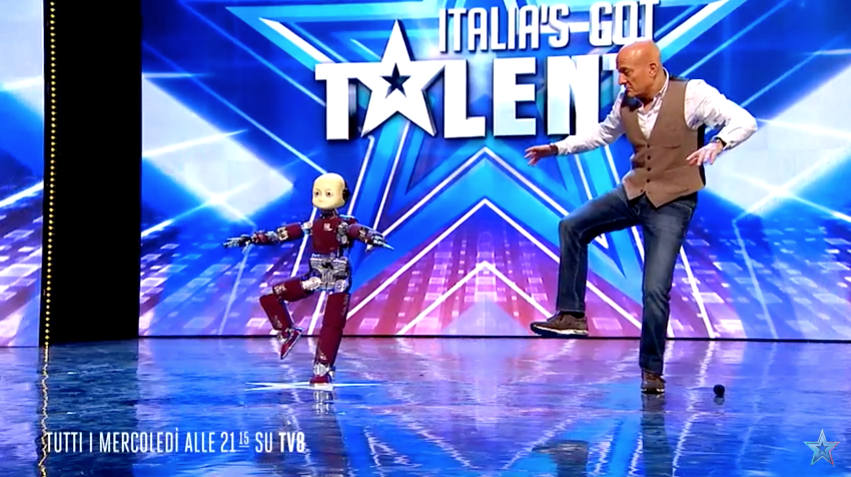
\includegraphics[height=.2\textwidth]{images/icub_igt}
  \caption{Right: an image of the most popular CoDyCo video, which reached
  almost two million views on youTube (statistics on the left).}
\end{figure}

Among the invitations as a speaker at international events it is worth citing the following:

\begin{enumerate}

\item Francesco Nori invited talk at the dissemination event Creative mornings. Talk: Interacting with Humans with iCub-humanoid. Dates: Location: May 22nd 2015. Milano, Italy.

\item Francesco Nori invited talk at Convegno NanoItaly, Roma, 21-24 settembre 2015. Talk: Force and motion capture system
based on distributed micro-accelerometers, gyros, force and tactile sensing. Date: 21 settembre 2015.

\item Talk by Elmar Rueckert, 02/2015 Probabilistic Inference and Modeling of Human Motor Skill Learning. Invited Talk. Workshop with Marc Toussaint’s group, Wolfram Burgard's group and Oliver Brock's group, Manigod, France.

\item  V. Padois. Robotique industrielle: \'evolution, enjeux et perspectives, January 2016. Invited talk at CNER/SERECT.

\item  Ivaldi, S. (12/2015) Human-robot interaction with iCub. Invited talk at University of Plymouth, by Samantha Adams and Angelo Cangelosi.

\item Babic, Jan. Human-in-the-loop control of robots for industrial assembly tasks : invited talk, Omron Keihanna Technology Innovation Center, 7th September 2015, Kyoto, Japan.

\end{enumerate} 

Live demonstration of the iCub have been performed at several international events.  Some of these events were sponsored by CoDyCo and the following is a non exhaustive list:

\begin{enumerate}

\item 12$^{th}$-14$^{th}$ March 2014. EU Robotics Forum Rovereto. \url{http://www.erf2014.eu/erf_home.jsp}.
\item 3$^{rd}$-6$^{th}$ June 2014. Automatica 2014, Munich, Germany. \url{http://www.nfm-automatica.de/2014/en/home.php}.
\item 3$^{rd}$-5$^{th}$ October 2014. European Maker Faire, Roma, Italy. \url{http://www.makerfairerome.eu/en/agenda2014/}. 
\item 18$^{th}$-20$^{th}$ November 2014. 2014 IEEE-RAS International Conference on Humanoid Robots (Humanoids 2014), Madrid, Spain. \url{http://www.humanoids2014.com}.

\end{enumerate} 

Among the invitations as a speaker at international events it is worth citing the following:

\begin{enumerate}

\item Francesco Nori: invited speaker at the Journées Nationales du GdR Robotique 2014, held at Grand amphith\'e\^atre du Centre Arts et M\`etiers ParisTech, 151-155 boulevard de l'Hôpital, 75013 Paris. 30 October 2014. \url{http://www.gdr-rob2014.org}.

\item Serena Ivaldi: invited speaker French-German-Japan Workshop on Humanoid and Legged robots. Social learning and engagement in human-humanoid interactions. \url{http://orb.iwr.uni-heidelberg.de/hlr2014/HLR14}.

\item Jan Babic: invited talk in Paris at the Université Pierre et Marie Curie. Synthesis of skilled robotic behaviour through human sensorimotor adaptation:  12$^th$ November 2014.

\item Jan Peters: keynote for the Learning by Demonstration Session Topic at the IEEE/RSJ International Conference on Intelligent Robots and Systems (IROS), Chicago, USA.

\item Jan Peters: invited plenary talk speaker at the 13th International Conference on Intelligent Autonomous Systems (IAS-13), Padua, Italy.

\item Vincent Padois: invited talk at the Cap Digital/Innorobo day about Robotics et Innovations. ``Issues and challenges of interactive robotics in complex industrial contexts''. Lyon, France - March 2014.

\item Michael Mistry: invited Lecturer at European Computational Motor Control Summer School. June 15$^th$-21$^st$, 2014.

\end{enumerate} 

Also, during the fourth year the CoDyCo consortium conducted the following 
 wide audience dissemination activities:
 
 \begin{enumerate}
 \item ``Technologies: les robots envahissent notre quotidien''
 May 26th, 2016: Reportage the for the daily evening news show ``Le Grand Soir 3'' on the national channel France 3. URL : \url{http://www.francetvinfo.fr/internet/technologies-les-robots-envahissent-notre-quotidien_1470757.html}.
 
 \item ``iCub on TgCom24''. October 17th, 2016. Live event with the iCub showing his balancing capabilities during
 a event connected to the Festival della Scienza.
 
 \item The iCub advanced balancing capabilities were on IEEE Spectrum Video Friday twice during 2016. 
 See the yoga++ video  
\url{https://goo.gl/2V3Uzn} and the footstep recovery  \url{https://goo.gl/b2sZmE}.

\item The iCub and CoDyco were on an Italian newspaper. \url{https://goo.gl/xJCrMG}.

 \end{enumerate}

\section{Impact and collaborations}

\begin{figure}
  \centering
    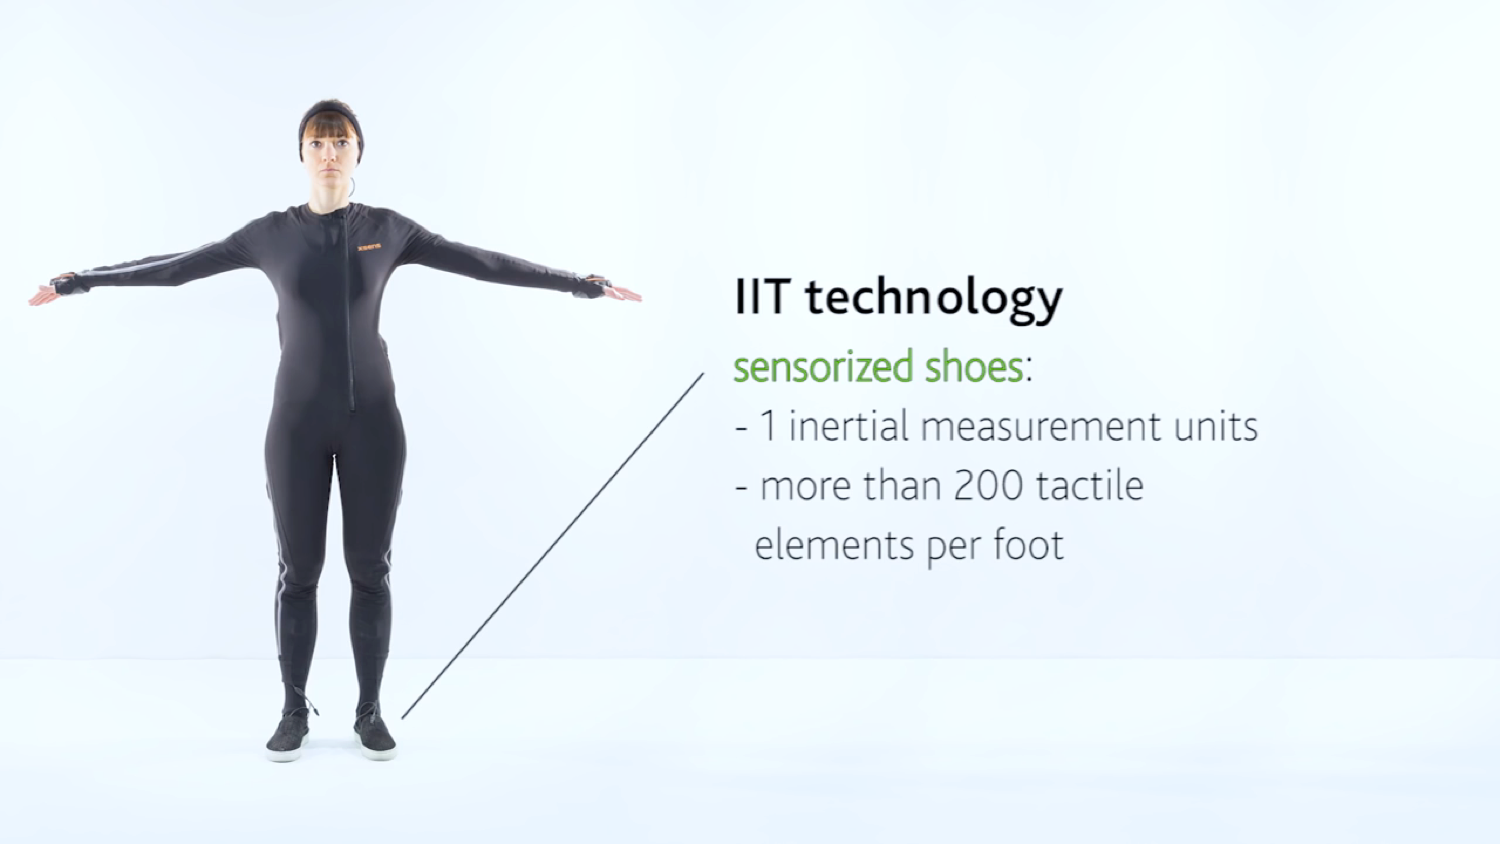
\includegraphics[height=.25\textwidth]{images/AnDy-IIT}
    \hspace{1cm}
    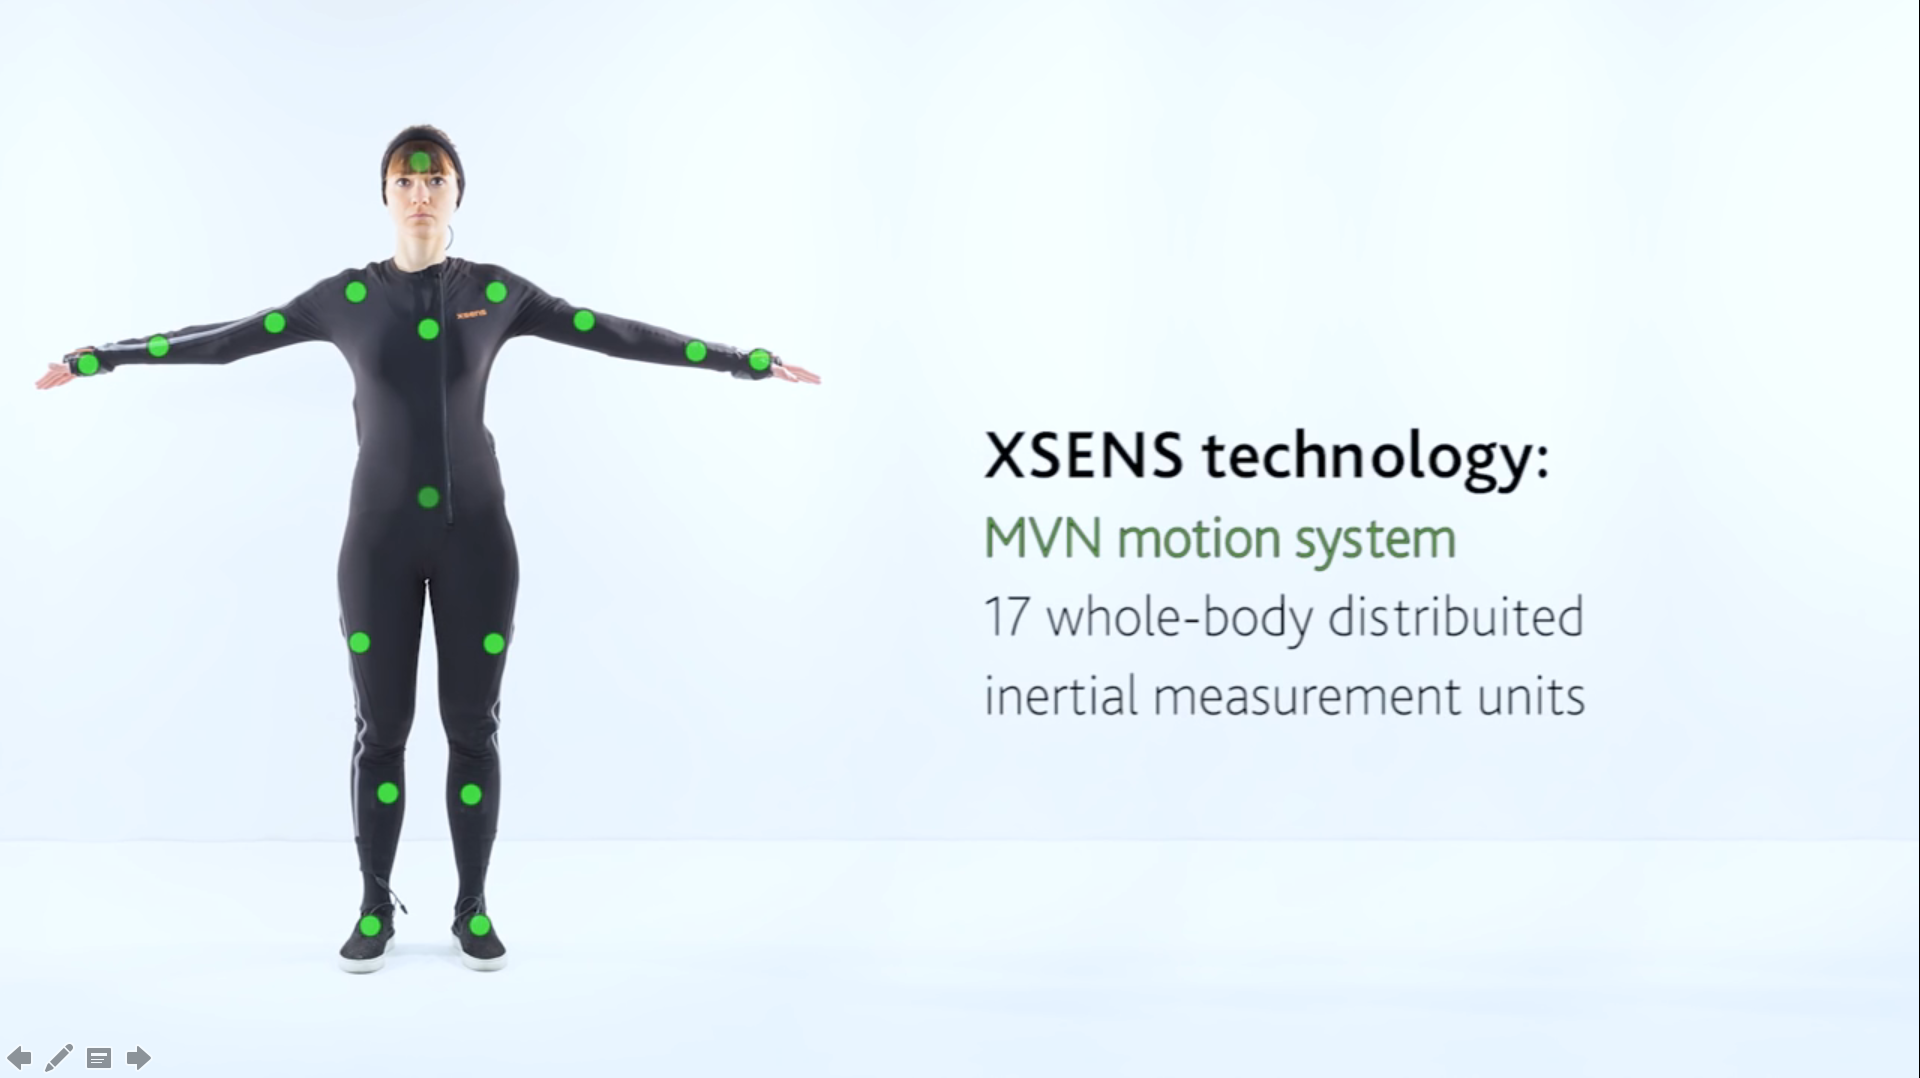
\includegraphics[height=.25\textwidth]{images/AnDy-XSENS}
  \caption{The figure shows the technology that resulted from the
  combination of a CoDyCo technology (tactile foot soles and real-time
  inverse dynamics computations) and a commercial technology
  (XSENS-MVN wearable motion capture system). The resulting technology
  is a fully wearable force and motion tracking system.}
 \label{fig:XSENS_IIT}
\end{figure}


The CoDyCo project is the prerequisite for impacting on industrial applications.
Its results and in particular those related to physical human-robot collaboration
fostered a number of applications related in the field of healthcare, rehabilitation
and safety at work (i.e. ergonomy). These ideas will be further investigated in 
the project An.Dy - Advancing Anticipatory Behaviors in Dyadic Human-Robot Collaboration,
which has received funding from the European Union's Horizon 2020 Research and Innovation Programme under Grant Agreement No. 731540.

Moreover, an industrial collaboration between IIT and XSENS started at the end of 
2015. This collaboration (see Figure \ref{fig:XSENS_IIT}) combines technologies
developed by IIT (the inverse dynamics algorithm and the tactile sensor) 
with commercial technologies (XSENS - MVN wearable motion capture system)
to obtain a new real-time system for simultaneous force and motion tracking.

\subsubsection{Stakeholders involvement}

Within the scope of the new funded EU project, a number of stakeholders were
involved through the creation of the end-users advisory board. Involved companies 
include representatives from all possible applications of the developed technology:

\begin{itemize}
\item \textbf{ABB} (manufacturing, safety in pHRI, standardization): Hao Ding (Senior Scientist at ABB Corporate Research).
\item \textbf{AC Milan} (sport analysis): Luca Gatti (Business Development MilanLab at AC Milan) and Daniele Tognaccini (project leader milanlab at AC Milan).
\item \textbf{INRS} (safety at work): Didier Baptiste (Scientific Director), Jean Theurel, Laurent Claudon.
\item \textbf{TECNALIA} (wearable sensing): Jan Veneman.
\item \textbf{CEA} (collaborative robotics, exoskeletons): Yvan Measson.
\item \textbf{FCA Group} (automotive, previously known as FIAT): Fabrizio Cencetti (Head of Environment, Health and Safety)
\item \textbf{Sapienza University of Rome}, Department of Medical and Surgical Sciences and Biotecnologies, Polo Pontino, Latina, Italy. Dr. Maria Serrao. 
\item \textbf{Daimler AG} (automotive, confirmed, terms under negotiation): Dr. Martin Manns (Integrated Production Validation).
\item \textbf{Fraunhofer FKIE} (security/ergonomics, confirmed, terms under negotiation): Dr. Thomas Alexander (Head of Human Factors Department).
\end{itemize}


\end{document}

%%% Local Variables:
%%% mode: latex
%%% TeX-master: t
%%% save-place: t
%%% End:
